
\pgfplotsset{
  compat=1.16,
  % load a colormap that already included black
  % (either at the beginning or at the end)
  colormap/blackwhite,
  /pgf/declare function={
      u(\x,\y) = (1+0.5*y*cos(x/2)))*cos(x);
      v(\x,\y) = (1+0.5*y*cos(x/2)))*sin(x);
      id(\x,\y)= 0.5*y;
      twist(\x,\y) = 0.5*y*sin(x/2);
  }
}


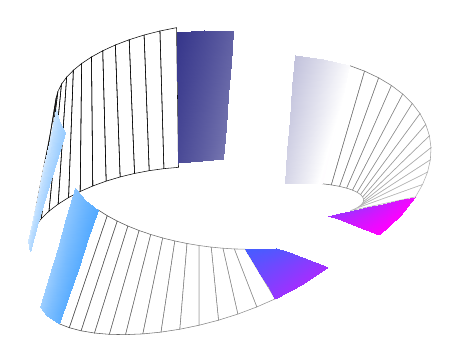
\begin{tikzpicture}
  \begin{axis}[
      hide axis,
      view={40}{40},
      domain=-145:180, % The domain needs to be adjusted manually, depending on the camera angle, unfortunately
  ]
  \addplot3 [
      mesh,
      point meta=x,
      samples=14,
      samples y=2,
      z buffer=sort,
      y domain=-0.5:0.5,
      line width=0.2pt,
      fill=white,
      domain=140:220,
  ] (
    {u(x,y)},
    {v(x,y)},
    {id(x,y)});

  \addplot3 [
      surf,
      point meta=x,
      samples=14,
      samples y=2,
      z buffer=sort,
      y domain=-0.5:0.5,
      line width=0.2pt,
      fill=white,
      domain=20:100,
  ] (
    {u(x,y)}+0.6,
    {v(x,y)},
    {twist(x,y)});

  \addplot3 [
      surf,
      point meta=x,
      samples=14,
      samples y=2,
      z buffer=sort,
      y domain=-0.5:0.5,
      line width=0.2pt,
      fill=white,
      domain=260:340,
  ] (
    {u(x,y)}+0.1,
    {v(x,y)},
    {twist(x,y)}-0.2);

  %top right gluing data
  \addplot3 [
      surf,
      colormap/violet,
      point meta=x,
      shader=interp,
      samples=3,
      samples y=5,
      z buffer=sort,
      y domain=-0.5:0.5,
      line width=0.2pt,
      domain=120:140,
  ] (
    {u(x,y)},
    {v(x,y)},
    {twist(x,y)});

  \addplot3 [
      surf,
      colormap/violet,
      point meta=x,
      shader=interp,
      samples=3,
      samples y=5,
      z buffer=sort,
      y domain=-0.5:0.5,
      line width=0.2pt,
      fill=white,
      domain=100:120,
  ] (
    {u(x,y)}+0.6,
    {v(x,y)},
    {twist(x,y)});
  
  %bottom right gluing data
  \addplot3 [
      surf,
      colormap/cool,
      point meta=x,
      shader=interp,
      samples=3,
      samples y=5,
      z buffer=sort,
      y domain=-0.5:0.5,
      line width=0.2pt,
      fill=white,
      domain=340:360,
  ] (
    {u(x,y)}+0.1,
    {v(x,y)},
    {twist(x,y)-0.2});
  \addplot3 [
      surf,
      colormap/cool,
      point meta=x,
      shader=interp,
      samples=3,
      samples y=5,
      z buffer=sort,
      y domain=-0.5:0.5,
      line width=0.2pt,
      fill=white,
      domain=0:20,
  ] (
    {u(x,y)}+0.6,
    {v(x,y)},
    {twist(x,y)});

  %top left gluing data
  \addplot3 [
      surf,
      colormap/cool,
      point meta=x,
      shader=interp ,
      samples=3,
      samples y=5,
      z buffer=sort,
      y domain=-0.5:0.5,
      line width=0.2pt,
      fill=white,
      domain=220:240,
  ] (
    {u(x,y)},
    {v(x,y)},
    {twist(x,y)});

  \addplot3 [
      surf,
      colormap/cool,
      point meta=x,
      shader=interp,
      samples=3,
      samples y=5,
      z buffer=sort,
      y domain=-0.5:0.5,
      line width=0.2pt,
      fill=white,
      domain=240:260,
  ] (
    {u(x,y)}+0.1,
    {v(x,y)},
    {twist(x,y)}-0.2);
    

  
  \end{axis}
  \end{tikzpicture}